\documentclass[journal]{IEEEtran}
\usepackage[a5paper, margin=10mm, onecolumn]{geometry}
\usepackage{tfrupee}
\usepackage{cite}
\usepackage{amsmath,amssymb,amsfonts,amsthm}
\usepackage{algorithmic}
\usepackage{graphicx}
\usepackage{textcomp}
\usepackage{xcolor}
\usepackage{listings}
\usepackage{enumitem}
\usepackage{mathtools}
\usepackage{gensymb}
\usepackage{comment}
\usepackage[breaklinks=true]{hyperref}
\usepackage{tkz-euclide}
\usepackage{longtable}
\usepackage{multirow}
\usepackage{hhline}
\usepackage{array}

\newcommand{\myvec}[1]{\begin{bmatrix}#1\end{bmatrix}}

\begin{document}
\title{3.2.1.2}
\author{EE24BTECH11004 - Ankit Jainar}
\maketitle

\textbf{Question:} \(5\) pencils and \(7\) pens together cost Rs.\(50\), whereas \(7\) pencils and \(5\) pens together cost Rs.\(46\). Find the cost of one pencil and that of one pen.\\

\section*{Solution:}
Let the cost of one pencil be denoted by \(x\) and the cost of one pen by \(y\).  
The situation can be described using the following system of linear equations:
\begin{align}
    5x + 7y &= 50, \tag{1} \\
    7x + 5y &= 46. \tag{2}
\end{align}

\section{Theoretical Solution}
We solve the above equations using elimination:
\begin{itemize}
    \item Multiply equation \((1)\) by \(5\) and equation \((2)\) by \(7\).
    \item Subtract the resulting equations to eliminate \(y\) and solve for \(x\).
    \item Substitute the value of \(x\) back into either equation to find \(y\).
\end{itemize}

Performing these steps:
\[
x = 3, \quad y = 5.
\]
\section{Numerical Method:}
\section{LU Decomposition to Solve the System}
We now solve the system of equations using LU decomposition.

\subsection{Matrix Form}
The system of equations can be expressed in matrix form as:
\begin{equation}
    \myvec{
    5 & 7 \\
    7 & 5
    } \myvec{x \\ y} = \myvec{50 \\ 46}.
\end{equation}
Here, the coefficient matrix is:
\begin{equation}
    A = \myvec
    {5 & 7 \\
    7 & 5}, \quad \vec{b} = \myvec{50 \\ 46}.
\end{equation}

\subsection{Step 1: Decomposing \(A\) into \(L\) and \(U\)}
The matrix \(A\) can be decomposed into:
\begin{equation}
    A = L \cdot U,
\end{equation}
where:
\begin{align}
    L &= \myvec{1 & 0 \\ \frac{7}{5} & 1}, \\
    U &= \myvec{5 & 7 \\ 0 & -\frac{14}{5}}.
\end{align}


\subsection*{Step 2: LU Factorization Using Update Equations}
Given a matrix \( \mathbf{A} \) of size \( n \times n \), LU decomposition is performed row by row and column by column. The update equations are as follows:  

\textbf{Step-by-Step Procedure:}
1. \textbf{Initialization:}  
   - Start by initializing \( \mathbf{L} \) as the identity matrix \( \mathbf{L} = \mathbf{I} \) and \( \mathbf{U} \) as a copy of \( \mathbf{A} \).

2. \textbf{Iterative Update:}  
   - For each pivot \( k = 1, 2, \ldots, n \):  
     - Compute the entries of \( U \) using the first update equation.  
     - Compute the entries of \( L \) using the second update equation.  

3. \textbf{Result:}  
   - After completing the iterations, the matrix \( \mathbf{A} \) is decomposed into \( \mathbf{L} \cdot \mathbf{U} \), where \( \mathbf{L} \) is a lower triangular matrix with ones on the diagonal, and \( \mathbf{U} \) is an upper triangular matrix.  

\subsection*{1. Update for \( U_{k,j} \) (Entries of \( U \))}
For each column \( j \geq k \), the entries of \( U \) in the \( k \)-th row are updated as:  
\[
U_{k,j} = A_{k,j} - \sum_{m=1}^{k-1} L_{k,m} \cdot U_{m,j}, \quad \text{for } j \geq k.
\]
This equation computes the elements of the upper triangular matrix \( \mathbf{U} \) by eliminating the lower triangular portion of the matrix.

\subsection*{2. Update for \( L_{i,k} \) (Entries of \( L \))}
For each row \( i > k \), the entries of \( L \) in the \( k \)-th column are updated as:  
\[
L_{i,k} = \frac{1}{U_{k,k}} \left( A_{i,k} - \sum_{m=1}^{k-1} L_{i,m} \cdot U_{m,k} \right), \quad \text{for } i > k.
\]
This equation computes the elements of the lower triangular matrix \( \mathbf{L} \), where each entry in the column is determined by the values in the rows above it.

\subsection*{LU Factorization of Matrix \( A \)}
We decompose \( A \) as:
\[
A = LU,
\]
where \( L \) is a lower triangular matrix and \( U \) is an upper triangular matrix.  
For the given example, we calculate \( L \) and \( U \) as follows:
\[
L = \begin{bmatrix} 1 & 0 \\ \frac{2}{3} & 1 \end{bmatrix}, \quad 
U = \begin{bmatrix} 3 & 2 \\ 0 & -\frac{13}{3} \end{bmatrix}.
\]

\subsection{Step 2: Forward Substitution}
The system \(A\vec{x} = \vec{b}\) is transformed into \(L \cdot U \cdot \vec{x} = \vec{b}\). Let \(\vec{y}\) satisfy \(L\vec{y} = \vec{b}\):
\begin{equation}
    \myvec{1 & 0 \\ \frac{7}{5} & 1} \myvec{y_1 \\ y_2} = \myvec{50 \\ 46}.
\end{equation}

Using forward substitution:
\begin{align}
    y_1 &= 50, \\
    \frac{7}{5}y_1 + y_2 &= 46 \implies y_2 = 46 - \frac{7}{5}(50) = -24.
\end{align}
Thus:
\begin{equation}
    \vec{y} = \myvec{50 \\ -24}.
\end{equation}

\subsection{Step 3: Back Substitution}
Next, solve \(U\vec{x} = \vec{y}\):
\begin{equation}
    \myvec{5 & 7 \\ 0 & -\frac{14}{5}} \myvec{x \\ y} = \myvec{50 \\ -24}.
\end{equation}

Using back substitution:
\begin{align}
    -\frac{14}{5}y &= -24 \implies y = 5, \\
    5x + 7(5) &= 50 \implies x = 3.
\end{align}

\subsection{Updated Equation:}
\begin{align}
    A\vec{x} &= L \cdot U \cdot \vec{x} = \vec{b}, \\
    A &= L \cdot U, \\
    L \cdot U \cdot \vec{x} &= \vec{b}, \\
    U \cdot \vec{x} &= \vec{y}, \\
    L \cdot \vec{y} &= \vec{b}.
\end{align}

\subsection{Final Answer}
The cost of one pencil is Rs.\(3\), and the cost of one pen is Rs.\(5\).

\begin{figure}[h!]
   \centering
   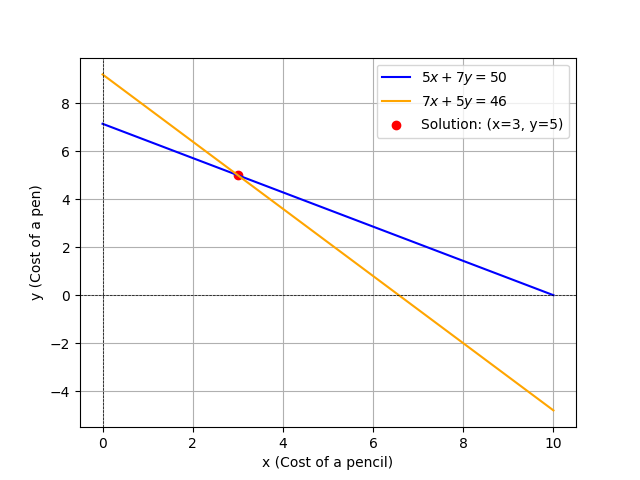
\includegraphics[width=0.7\columnwidth]{figs/fig.png}
    \caption{Graphical Representation of the Solution}
\end{figure}

\end{document}

